\section{THIẾT KẾ UI/UX CHO ỨNG DỤNG}
\subsection{Màn hình đăng nhập và đăng ký tài khoản}
Khi lần đầu vào ứng dụng, người dùng cần phải đăng nhập vào tài khoản đã được tạo. Người dùng cần nhập tên đăng nhập và mật khẩu của họ để xác thực, hoặc họ có thể đăng nhập thông qua bên thứ ba là Facebook, Google hoặc là Apple ID.\\
Nếu người dùng vẫn chưa có tài khoản, họ có thể đăng ký bằng cách ấn vào nút "Đăng ký" để được điều hướng sang giao diện đăng ký tài khoản. Sau khi người dùng đã đăng ký thành công tài khoản, ứng dụng sẽ điều hướng sang trang nhập thông tin cá nhân. Người dùng có thể nhập các trường như họ và tên, số điện thoại, địa chỉ hoặc là chọn nút "Bỏ qua" để tạm thời không nhập các thông tin này.
\begin{figure}[!htb]
\centering
   \begin{minipage}{0.32\textwidth}
     \centering
     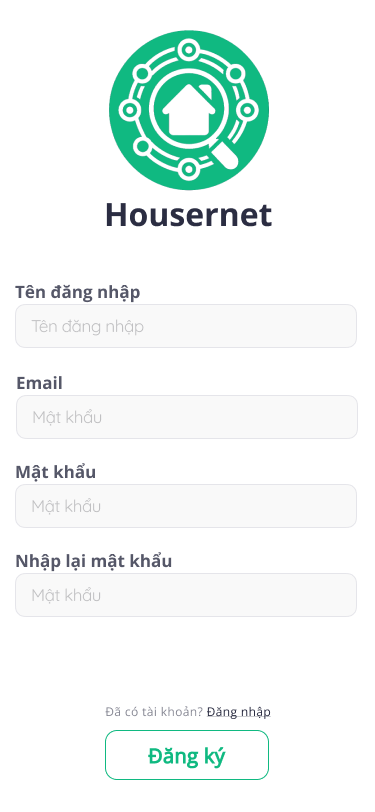
\includegraphics[width=1\linewidth]{Images/UI figma/Signup 1.png}
     \caption{Giao diện đăng ký với tài khoản và mật khẩu}
   \end{minipage}\hfill
   \begin{minipage}{0.32\textwidth}
     \centering
     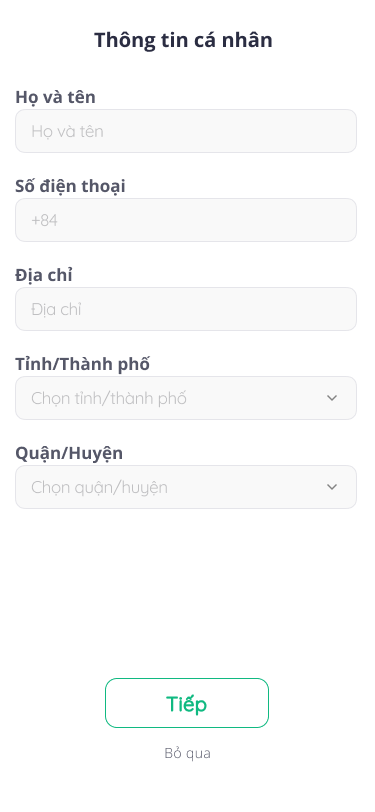
\includegraphics[width=1\linewidth]{Images/UI figma/Signup 2.png}
     \caption{Giao diện cung cấp thông tin cá nhân đăng ký}
   \end{minipage}\hfill
   \begin{minipage}{0.32\textwidth}
     \centering
     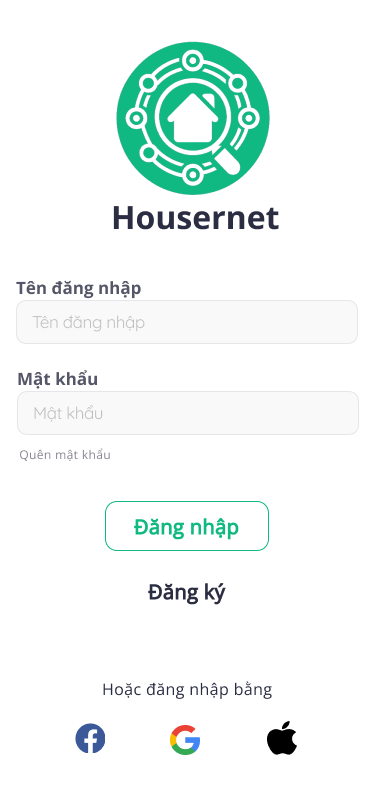
\includegraphics[width=1\linewidth]{Images/UI figma/Login}
     \caption{Giao diện đăng nhập}
   \end{minipage}
\end{figure}
\newpage
\subsection{Màn hình quên mật khẩu}
Housernet cung cấp chức năng đặt lại mật khẩu trong trường hợp người dùng quên mật khẩu. Người dùng có thể đặt lại mật khẩu bằng cách ấn vào chữ "Quên mật khẩu" trong màn hình đăng nhập.
\begin{figure}[H]
    \centering
    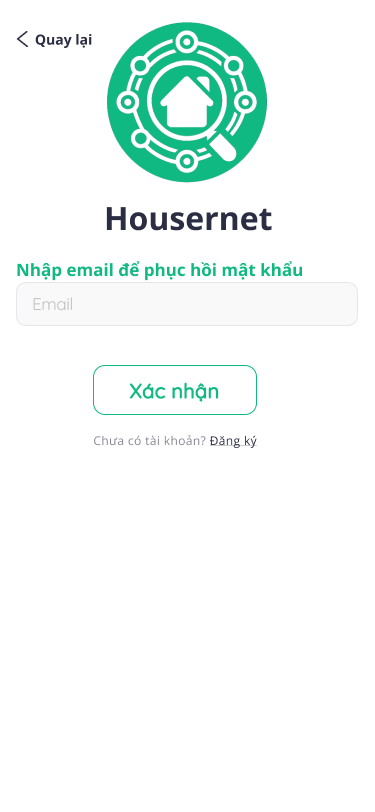
\includegraphics[width=0.33\textwidth]{Images/UI figma/Reset Password.png}
    \caption{Giao diện đặt lại mật khẩu}
\end{figure}
\newpage
\subsection{Màn hình chính}
Màn hình chính sẽ cung cấp các chức năng chính như:
\begin{itemize}
    \item Hiển thị danh sách nhà ở gần vị trí người dùng cung cấp
    \item Hiển thị danh sách nhà phù hợp với người dùng
    \item Tìm kiếm nhà bằng từ khóa như tên hoặc địa chỉ
    \item Cung cấp bộ lọc các nhà thỏa điều kiện.
\end{itemize}
Ngoài ra, tại góc dưới của màn hình chính còn có một thanh điều hướng có chức năng di chuyển đến các màn hình cài đặt và tài khoản.
\begin{figure}[H]
    \centering
    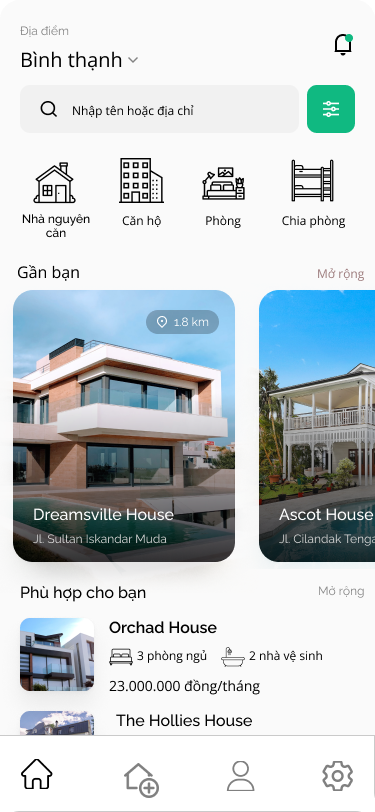
\includegraphics[width=0.33\textwidth]{Images/UI figma/Full home screen.png}
    \caption{Giao diện màn hình chính}
\end{figure}
\newpage
\subsection{Bộ lọc tìm kiếm nhà trọ}
Người dùng có thể sử dụng bộ lọc để lọc ra các kết quả cho nhà phù hợp điều kiện. Để có thể dùng bộ lọc, người dùng cần ấn vào nút lọc nằm cạnh bên phải thanh tìm kiếm tại màn hình chính. Bộ lọc bao gồm:
\begin{itemize}
    \item Loại, diện tích, số phòng: có thể ấn chọn 1 trong 4 loại
    \item Khu vực: Chọn khu vực như tỉnh/thành, quận/huyện hoặc phường/xã
    \item Giá: có thể kéo để chọn khoảng giá phù hợp
    \item Tiện ích: có thể chọn 1 hoặc nhiều tiện ích
\end{itemize}
\begin{figure}[!htb]
\centering
   \begin{minipage}{0.32\textwidth}
     \centering
     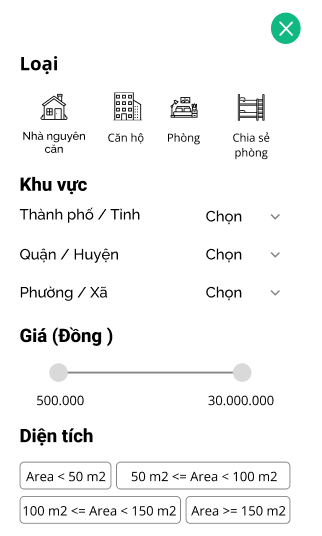
\includegraphics[width=1\linewidth]{Images/UI figma/Frame 1.png}
     \caption{Giao diện bộ lọc tìm kiếm nhà trọ}
   \end{minipage}\hspace{1cm}
   \begin{minipage}{0.32\textwidth}
     \centering
     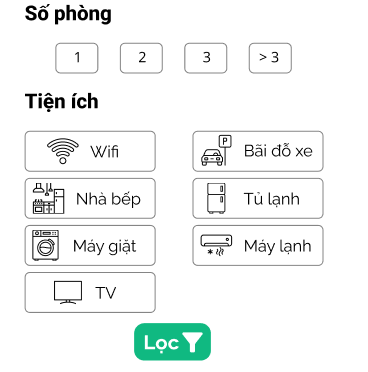
\includegraphics[width=1\linewidth]{Images/UI figma/Frame 2.png}
     \caption{Giao diện bộ lọc tìm kiếm nhà trọ (tiếp theo)}
   \end{minipage}
\end{figure}
\newpage
\subsection{Màn hình hồ sơ người dùng}
Người dùng có thể di chuyển đến màn hình tài khoản thông qua thanh điều hướng phía dưới trang chính. Tại đây người dùng có thể xem và điều chỉnh thông tin cá nhân hoặc là đăng xuất.
\begin{figure}[!htb]
    \centering
    \begin{minipage}{0.32\textwidth}
     \centering
     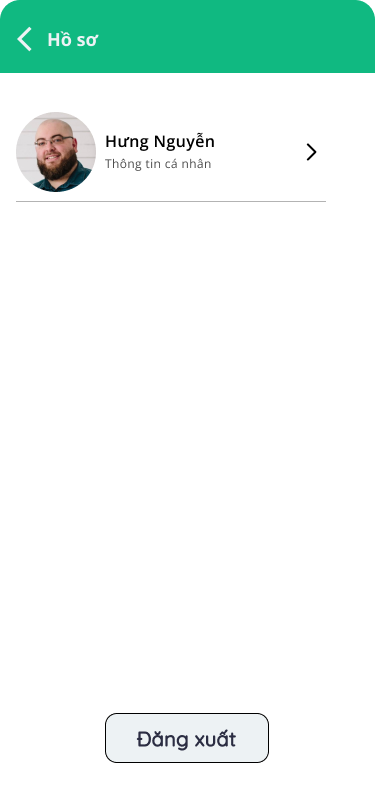
\includegraphics[width=1.06\linewidth]{Images/UI figma/Profile.png}
     \caption{Giao diện hồ sơ người dùng}
    \end{minipage}\hspace{1cm}
    \begin{minipage}{0.32\textwidth}
     \centering
     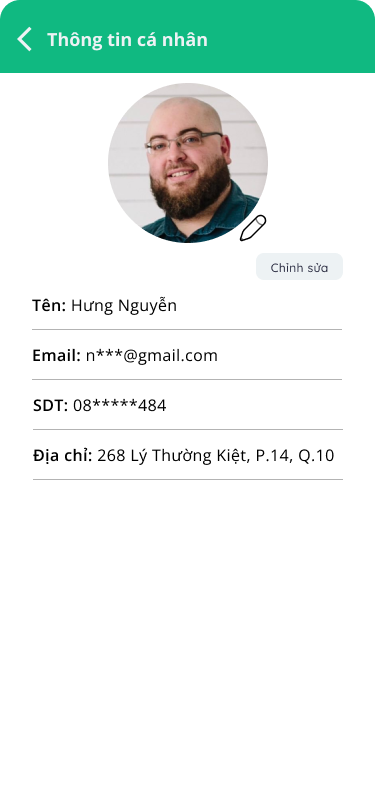
\includegraphics[width=1\linewidth]{Images/UI figma/Profile - Detail.png}
     \caption{Giao diện hồ sơ người dùng và thông tin cá nhân}
    \end{minipage}
\end{figure}
\newpage
\subsection{Đăng tải nhà trọ}
Chủ trọ có thể đăng tải nhà trọ để công khai thông tin nhà trọ lên ứng dụng bằng cách ấn vào nút "Đăng tải" tại giao diện quản lý nhà trọ. Để đăng tải, chủ trọ có thể chọn một nhà trọ đã có sẵn và ấn nút "Tiếp", lúc này ứng dụng sẽ tự động điền các thông tin đã có sẵn của nhà trọ và chủ trọ có thể sửa lại hoặc thêm các thông tin thêm như hình ảnh hoặc các tiện ích của nhà trọ. Sau khi chủ trọ ấn nút "Đăng tải" thì ứng dụng sẽ hiển thị thông báo thành công và chủ trọ có thể ấn nút "Quay về" để trở về màn hình chính.
\begin{figure}[!htb]
\centering
   \begin{minipage}{0.32\textwidth}
     \centering
     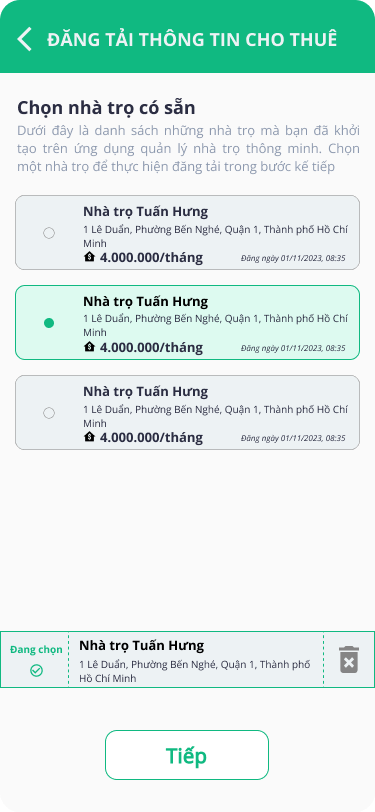
\includegraphics[width=1\linewidth]{Images/UI figma/Upload Rooming House 1.png}
     \caption{Giao diện chọn danh sách nhà trọ có sẵn}
   \end{minipage}\hfill
   \begin{minipage}{0.32\textwidth}
     \centering
     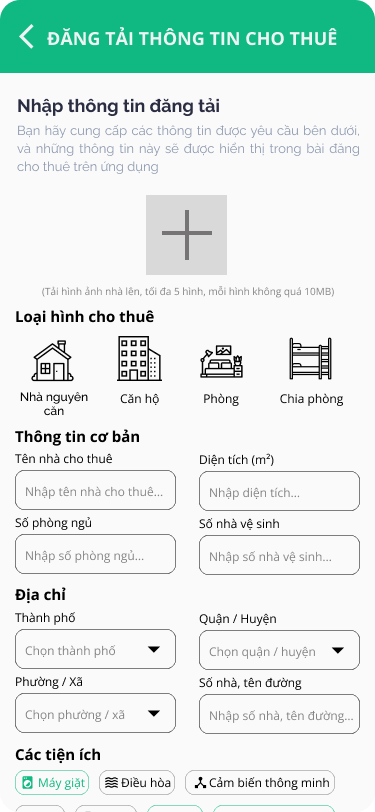
\includegraphics[width=1\linewidth]{Images/UI figma/Upload Rooming House 2.png}
     \caption{Giao diện nhập thông tin đăng tải nhà trọ}
   \end{minipage}\hfill
   \begin{minipage}{0.32\textwidth}
     \centering
     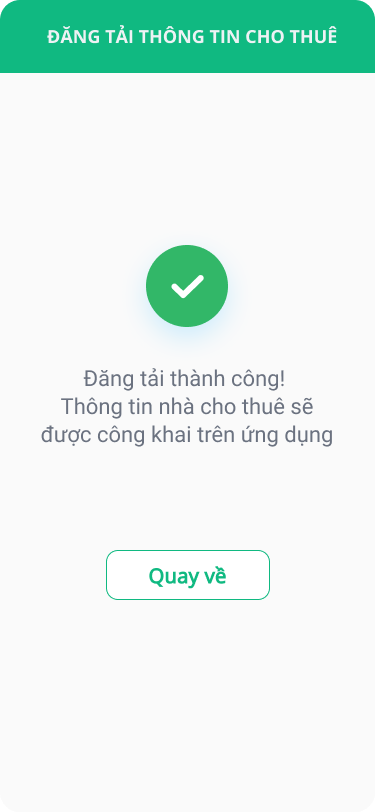
\includegraphics[width=1\linewidth]{Images/UI figma/Upload Rooming House 3.png}
     \caption{Giao diện đăng tải nhà trọ thành công}
   \end{minipage}
\end{figure}
\newpage
\subsection{Quản lý nhà trọ}
Người dùng có thể di chuyển sang màn hình này thông qua thanh điều hướng phía dưới màn hình chính. Tại đây, người dùng có thể xem danh sách cái nhà đã đăng bài và có thể thao tác chỉnh sửa cũng như gỡ bỏ bài đăng đó. Ngoài ra người dùng còn có thể tạo bài đăng nhà trọ bằng cách ấn vào nút "Đăng tải" hoặc thêm một nhà trọ mới bằng nút "Thêm nhà trọ".
\begin{figure}[!htb]
\centering
   \begin{minipage}{0.32\textwidth}
     \centering
     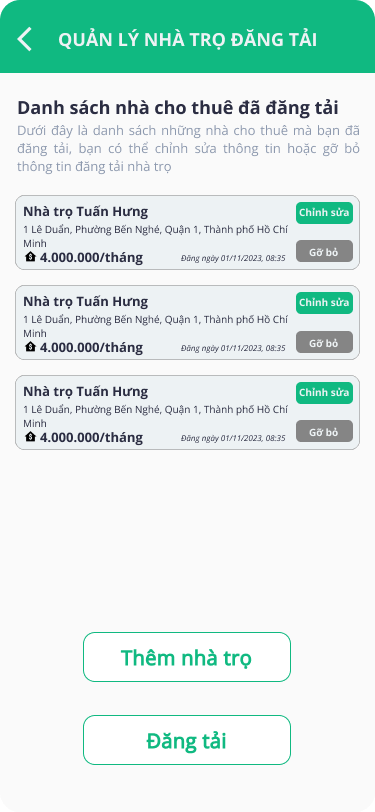
\includegraphics[width=1\linewidth]{Images/UI figma/Upload Rooming House 5.png}
     \caption{Giao diện chọn danh sách nhà trọ đã đăng}
   \end{minipage}\hfill
   \begin{minipage}{0.32\textwidth}
     \centering
     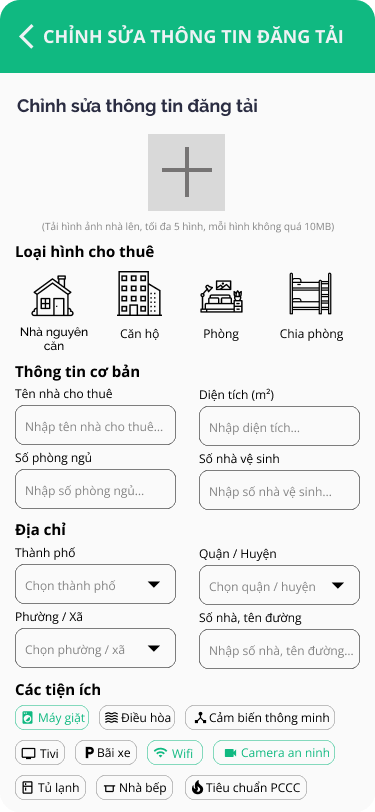
\includegraphics[width=1\linewidth]{Images/UI figma/Upload Rooming House 7.png}
     \caption{Giao diện chỉnh sửa thông tin đăng tải nhà trọ}
   \end{minipage}\hfill
   \begin{minipage}{0.32\textwidth}
     \centering
     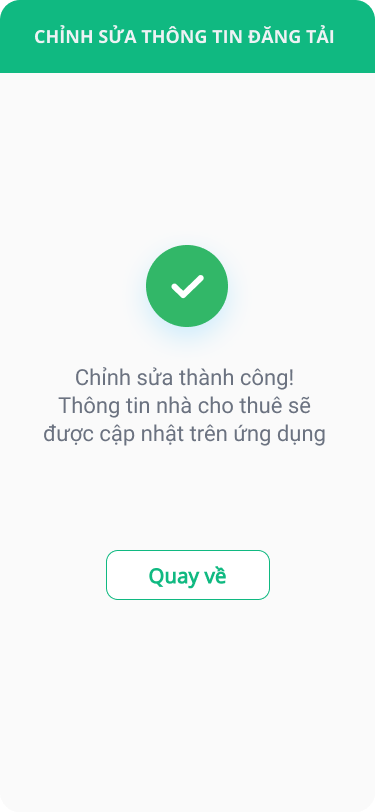
\includegraphics[width=1\linewidth]{Images/UI figma/Upload Rooming House 6.png}
     \caption{Giao diện chỉnh sửa nhà trọ thành công}
   \end{minipage}
\end{figure}

